%% BioMed_Central_Tex_Template_v1.06
%%                                      %
%  bmc_article.tex            ver: 1.06 %
%                                       %

%%IMPORTANT: do not delete the first line of this template
%%It must be present to enable the BMC Submission system to
%%recognise this template!!

%%%%%%%%%%%%%%%%%%%%%%%%%%%%%%%%%%%%%%%%%
%%                                     %%
%%  LaTeX template for BioMed Central  %%
%%     journal article submissions     %%
%%                                     %%
%%          <8 June 2012>              %%
%%                                     %%
%%                                     %%
%%%%%%%%%%%%%%%%%%%%%%%%%%%%%%%%%%%%%%%%%


%%%%%%%%%%%%%%%%%%%%%%%%%%%%%%%%%%%%%%%%%%%%%%%%%%%%%%%%%%%%%%%%%%%%%
%%                                                                 %%
%% For instructions on how to fill out this Tex template           %%
%% document please refer to Readme.html and the instructions for   %%
%% authors page on the biomed central website                      %%
%% http://www.biomedcentral.com/info/authors/                      %%
%%                                                                 %%
%% Please do not use \input{...} to include other tex files.       %%
%% Submit your LaTeX manuscript as one .tex document.              %%
%%                                                                 %%
%% All additional figures and files should be attached             %%
%% separately and not embedded in the \TeX\ document itself.       %%
%%                                                                 %%
%% BioMed Central currently use the MikTex distribution of         %%
%% TeX for Windows) of TeX and LaTeX.  This is available from      %%
%% http://www.miktex.org                                           %%
%%                                                                 %%
%%%%%%%%%%%%%%%%%%%%%%%%%%%%%%%%%%%%%%%%%%%%%%%%%%%%%%%%%%%%%%%%%%%%%

%%% additional documentclass options:
%  [doublespacing]
%  [linenumbers]   - put the line numbers on margins

%%% loading packages, author definitions

%\documentclass[twocolumn]{bmcart}% uncomment this for twocolumn layout and comment line below
\documentclass{bmcart}

%%% Load packages
\usepackage{amsthm,amsmath,amssymb,amsfonts}
\usepackage{algorithm,algorithmic}
%\RequirePackage{natbib}
%\RequirePackage[authoryear]{natbib}% uncomment this for author-year bibliography
\usepackage{graphicx}
\usepackage{tabularx}
\usepackage{multirow}
\usepackage{paralist}
\usepackage{gensymb}
\RequirePackage{hyperref}
\usepackage[utf8]{inputenc} %unicode support
%\usepackage[applemac]{inputenc} %applemac support if unicode package fails
%\usepackage[latin1]{inputenc} %UNIX support if unicode package fails

%%%%%%%%%%%%%%%%%%%%%%%%%%%%%%%%%%%%%%%%%%%%%%%%%
%%                                             %%
%%  If you wish to display your graphics for   %%
%%  your own use using includegraphic or       %%
%%  includegraphics, then comment out the      %%
%%  following two lines of code.               %%
%%  NB: These line *must* be included when     %%
%%  submitting to BMC.                         %%
%%  All figure files must be submitted as      %%
%%  separate graphics through the BMC          %%
%%  submission process, not included in the    %%
%%  submitted article.                         %%
%%                                             %%
%%%%%%%%%%%%%%%%%%%%%%%%%%%%%%%%%%%%%%%%%%%%%%%%%

%\def\includegraphic{}
%\def\includegraphics{}


%%% Put your definitions there:
\startlocaldefs
\newcommand{\tickYes}{\checkmark}

\newenvironment{Algorithm}[1]{\begin{minipage}{1\textwidth}\centering\begin{minipage}{#1}\begin{algorithm}[H]}
{\end{algorithm}\vspace{0.1cm}\end{minipage}\end{minipage}}

\newcommand{\INDSTATE}[1][1]{\STATE\hspace{#1\algorithmicindent}}
\newcommand{\indItem}{\setlength\itemindent{25pt}\item}

\endlocaldefs


%%% Begin ...
\begin{document}

%%% Start of article front matter
\begin{frontmatter}

\begin{fmbox}
\dochead{Research}

%%%%%%%%%%%%%%%%%%%%%%%%%%%%%%%%%%%%%%%%%%%%%%
%%                                          %%
%% Enter the title of your article here     %%
%%                                          %%
%%%%%%%%%%%%%%%%%%%%%%%%%%%%%%%%%%%%%%%%%%%%%%

\title{Determining Device Position through Minimal User Input}

%%%%%%%%%%%%%%%%%%%%%%%%%%%%%%%%%%%%%%%%%%%%%%
%%                                          %%
%% Enter the authors here                   %%
%%                                          %%
%% Specify information, if available,       %%
%% in the form:                             %%
%%   <key>={<id1>,<id2>}                    %%
%%   <key>=                                 %%
%% Comment or delete the keys which are     %%
%% not used. Repeat \author command as much %%
%% as required.                             %%
%%                                          %%
%%%%%%%%%%%%%%%%%%%%%%%%%%%%%%%%%%%%%%%%%%%%%%

\author[
   addressref={aff1},                   % id's of addresses, e.g. {aff1,aff2}
   corref={aff1},                       % id of corresponding address, if any
%   noteref={n1},                        % id's of article notes, if any
   email={j.a.mcnaughton@durham.ac.uk}   % email address
]{\inits{JM}\fnm{James} \snm{McNaughton}}
\author[
   addressref={aff2},
   email={tcrick@cardiffmet.ac.uk}
]{\inits{TC}\fnm{Tom} \snm{Crick}}
\author[
   addressref={aff1},
   email={a.hatch@durham.ac.uk}
]{\inits{AH}\fnm{Andrew} \snm{Hatch}}

%%%%%%%%%%%%%%%%%%%%%%%%%%%%%%%%%%%%%%%%%%%%%%
%%                                          %%
%% Enter the authors' addresses here        %%
%%                                          %%
%% Repeat \address commands as much as      %%
%% required.                                %%
%%                                          %%
%%%%%%%%%%%%%%%%%%%%%%%%%%%%%%%%%%%%%%%%%%%%%%


\address[id=aff1]{%                           % unique id
  \orgname{School of Education, Durham University}, % university, etc
  \street{South Road},                     %
  \postcode{DH1 3LE}                                % post or zip code
  \city{Durham},                              % city
  \cny{UK}                                    % country
}
\address[id=aff2]{%
  \orgname{Department of Computing \& Information Systems, Cardiff Metropolitan University},
  \street{Western Avenue},
  \postcode{CF5 2YB}
  \city{Cardiff},
  \cny{UK}
}

%%%%%%%%%%%%%%%%%%%%%%%%%%%%%%%%%%%%%%%%%%%%%%
%%                                          %%
%% Enter short notes here                   %%
%%                                          %%
%% Short notes will be after addresses      %%
%% on first page.                           %%
%%                                          %%
%%%%%%%%%%%%%%%%%%%%%%%%%%%%%%%%%%%%%%%%%%%%%%

\begin{artnotes}
%\note{Sample of title note}     % note to the article
%\note[id=n1]{Equal contributor} % note, connected to author
\end{artnotes}

\end{fmbox}% comment this for two column layout

%%%%%%%%%%%%%%%%%%%%%%%%%%%%%%%%%%%%%%%%%%%%%%
%%                                          %%
%% The Abstract begins here                 %%
%%                                          %%
%% Please refer to the Instructions for     %%
%% authors on http://www.biomedcentral.com  %%
%% and include the section headings         %%
%% accordingly for your article type.       %%
%%                                          %%
%%%%%%%%%%%%%%%%%%%%%%%%%%%%%%%%%%%%%%%%%%%%%%

\begin{abstractbox}

\begin{abstract} % abstract
% \parttitle{First part title} %if any
% Text for this section.
% \parttitle{Second part title} %if any
% Text for this section.

In many co-located, collaborative systems there is a need for the devices used to be informed of the physical positions of their networked counterparts.
This paper presents a novel method of utilising users' judgement of direction to attain the location and orientation of a touch interface.
The technique requires a user to draw several arrows on an interface which point towards physical landmarks in an environment.
This allows for the setup of interface locations in a way which is: \begin{inparaenum}[(i)] \item quick, \item inexpensive, \item not encumbering and \item capable of being performed despite obstructions in the environment\end{inparaenum}.
A user study is presented which investigates what influence a user's accuracy has on the technique's resulting calculated location of an interface.
The study reveals that the magnitude of a user's inaccuracies is proportional to the size of the error in the result and that there is no improvement in user accuracy with practice.
\end{abstract}

%%%%%%%%%%%%%%%%%%%%%%%%%%%%%%%%%%%%%%%%%%%%%%
%%                                          %%
%% The keywords begin here                  %%
%%                                          %%
%% Put each keyword in separate \kwd{}.     %%
%%                                          %%
%%%%%%%%%%%%%%%%%%%%%%%%%%%%%%%%%%%%%%%%%%%%%%

\begin{keyword}
\kwd{Minimising User Input, positions, locating, physical environments, configuration, HCI}
\end{keyword}

% MSC classifications codes, if any
%\begin{keyword}[class=AMS]
%\kwd[Primary ]{}
%\kwd{}
%\kwd[; secondary ]{}
%\end{keyword}

\end{abstractbox}
%
%\end{fmbox}% uncomment this for twcolumn layout

\end{frontmatter}

%%%%%%%%%%%%%%%%%%%%%%%%%%%%%%%%%%%%%%%%%%%%%%
%%                                          %%
%% The Main Body begins here                %%
%%                                          %%
%% Please refer to the instructions for     %%
%% authors on:                              %%
%% http://www.biomedcentral.com/info/authors%%
%% and include the section headings         %%
%% accordingly for your article type.       %%
%%                                          %%
%% See the Results and Discussion section   %%
%% for details on how to create sub-sections%%
%%                                          %%
%% use \cite{...} to cite references        %%
%%  \cite{koon} and                         %%
%%  \cite{oreg,khar,zvai,xjon,schn,pond}    %%
%%  \nocite{smith,marg,hunn,advi,koha,mouse}%%
%%                                          %%
%%%%%%%%%%%%%%%%%%%%%%%%%%%%%%%%%%%%%%%%%%%%%%

%%%%%%%%%%%%%%%%%%%%%%%%% start of article main body
% <put your article body there>

%%%%%%%%%%%%%%%%
%% Background %%
%%

\section*{Introduction}\label{sec:intro}

Direct-touch interfaces provide an effective digital medium in which people can collaborate on various tasks~\cite{Marshall2008}. 
Research regarding collaboration on direct-touch interfaces is generally focused on collaboration between multiple participants across a single interface~\cite{Piper2009,Rick2009,Ryall2006a}. 
However, when multiple interfaces capable of interacting with each other are used, an opportunity arises for collaboration between users interacting with different interfaces.
This use of multiple interfaces in a shared environment can be beneficial for collaboration~\cite{Wallace2008a,Wallace2009}.

The physical locations of interfaces can be used to aid tasks involving interaction between networked devices.
For example, the Interactive Workspaces project~\cite{Johanson2002} generates a map of interface locations.
This map is used to facilitate collaboration between the multiple interfaces.
Users can pass materials between the interfaces using their knowledge of their physical positions.
When a material transfer is initiated the system can use the direction defined by the user and the generated map to find the interface the materials should be sent to.

% TODO Will need a new graphic here as we used this one before.
\begin{figure}[h!]
   \centering
   \caption{An example of how content items can be transferred between linked interfaces using flicking.}
   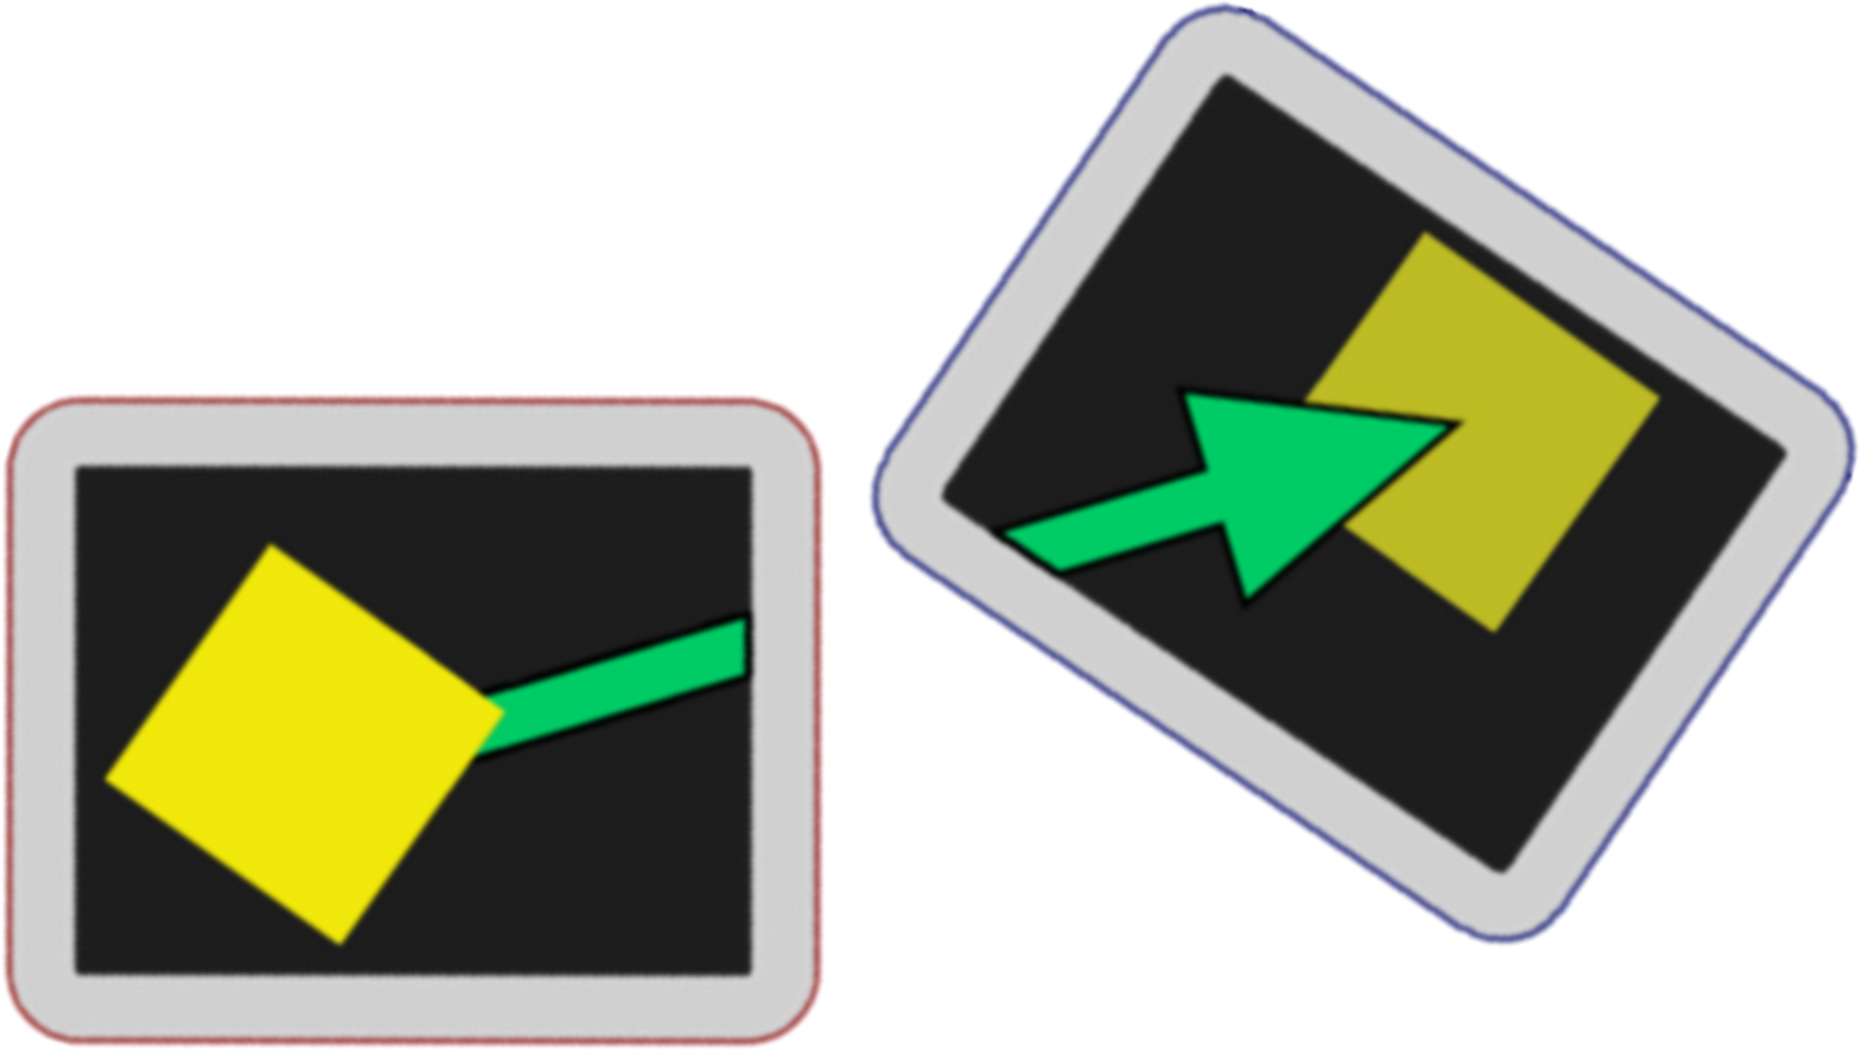
\includegraphics[width=0.6\textwidth]{figures/flicking.png}
   \label{fig:flick}
\end{figure}

Activities of content sharing in multi-interface environments are becoming more common~\cite{Nacenta2009}.
Another example of where the knowledge of interface locations facilitates the passing of materials between separate devices originates from the {\emph{SynergyNet}} project~\cite{Burd2009}.
The software framework built for {\emph{SynergyNet}} is intended for use on direct-touch interfaces, specifically multi-touch tabletops.
This allows the system to allow users to perform a flicking motion~\cite{Reetz2006} to transfer content.
Users flick a content item in the direction of the interface they wish to send content to.
The item travels off the side of the source interface and appears on the target interface as shown in Figure \ref{fig:flick}.
When the item arrives on the target interface, the framework can use its knowledge of the interface locations to ensure the item travels into view from the direction of the source interface. % TODO Reference to Remote collab paper here.
This is intended to aid users in identifying where newly arrived content items were sent from.

Both the {\emph{Interactive Workspaces}}~\cite{Johanson2002} and {\emph{SynergyNet}} projects showcase the need for an interface to have knowledge of its location relative to networked interfaces surrounding it.
Another example of the benefits of an interface knowing its location originates from a system which uses multiple projectors where projected outputs overlap.
The outputs are seamlessly stitched together by the system to give the appearance of a single projection.
In order for this to be achieved the system must have information regarding the relative positions of each projected output.
The stitching of multiple projector outputs to create large public displays is becoming much more frequent~\cite{Jones2011}.
Each system which utilises the stitching of visual outputs needs a method of attaining their locations.

With systems requiring knowledge of the locations of their interfaces, a method of obtaining this information is needed.
It is possible to measure the location and orientation of an interface using physical tools like rulers and protractors. 
Because of the time consuming nature of this manual measurement strategy it is best suited for an environment in which the interfaces remain in a fixed position for long periods of time.

However, there are scenarios in which the interfaces may be moved on a regular basis.
For example, the {\emph{SynergyNet}} project is intended for classroom environments.
These classroom environments are physical spaces in which furniture is frequently moved or rearranged to accommodate different learning activities during the course of a day~\cite{Tiburcio2005}.
Therefore, it is likely that any interfaces in the environment used by the system will not remain in fixed positions.
Measuring the locations and angles of each interface in the environment directly (i.e. with measuring tapes, rulers and/or protractors), then inputting this information into the system will take time on every reconfiguration of the environment.
In this time the system will not function as intended because its knowledge of interface positions will be incorrect.

Incorrect knowledge of interface positions is problematic for systems which use the information to stitch multiple visual outputs~\cite{Dietz2004,Jones2011}.
The image displayed by a repositioned interface would no longer align with the output from other linked interfaces and therefore would not be appropriately stitched.

Therefore, a method of obtaining the position of an interface quickly, without the need for time consuming measurements, is required.


\section*{Background}\label{sec:related}

Obtaining the position of an interface can be achieved through technological means.
The use of RFID chips~\cite{Ni2004} is one such technological approach.
These devices are inexpensive and can be used to get the positional information of the object they are attached to.
However, the accuracy of locations given by RFID chips is dependent on the number of sensors in an environment.
Despite the relatively low cost of the chips, the large number of sensors needed for accurate readings can be expensive.
Also, the addition of more sensors requires the system to spend more time compiling the positional information for each RFID chip detected~\cite{Ni2004}.
The same trade-off between expense and accuracy is also present for similar technologies using electro-magnetic waves, such as Wi-Fi~\cite{Cheng2005}.

Infra-red sensors can be used to attain the locations of interfaces~\cite{Kortuem2005}.
By detecting the relative location and strength of known infra-red light sources, a device with infra-red sensors can determine its position.
However, the technology is very sensitive and small changes in the light level can result in the calculated location varying from the sensors' actual locations to a large extent~\cite{Kortuem2005}.
This technology can also be affected by obstruction.
An object blocking an infra-red sensor's view of one or more infra-red light sources can result in the system obtaining incorrect positional information.
Therefore, for this technology to be used in a system, the environment must be clear of obstruction and have a consistent light level.
These two restraints make this technology unsuitable for a number of potential usage scenarios.

Visible light can be used for detecting the location of an interface~\cite{Lee2004}.
Using light sensing technology, an interface can detect its location by using patterns projected from a light source.
However, similar to infra-red sensors, these visible light sensors require a clear view of as much of the projected light pattern as possible.
If obstructed, a sensor's reading would result an inaccurate calculation of its location.

Visual markers called fiducials~\cite{Bose1990}, which are often used in augmented reality systems, could also be used for obtaining the position of an interface.
A camera is used to identify and locate the markers which each carry a unique pattern recognisable by machine vision.
Several markers positioned on or around an interface could be located by a fiducial recognition system.
However, this technology requires a clear line of sight between the camera and the fiducials.
Like other location sensing technologies~\cite{Lee2004,Kortuem2005,Ni2004}, obstructions around the interface can cause inaccurate results.

When attempting to attain the location of an interface, an alternative to the use of sensing technologies is to utilise a technique driven by user input.
An example of this alternative method is where users measure the locations of the interface directly and input the information into the system through text entry. 
User inputs do have the disadvantage of relying on the accuracy of the users whereas sensing technologies can be relied on to be precise to a certain extent.
The accuracy of users can be influenced by a range of factors which would not affect the accuracy of sensing technologies, such as the magnitude of the distances being measured~\cite{Al-Imam2006}.
An inaccurate user-generated measurement, input as part of a location determining technique, would result in the calculated position of the interface being incorrect.
Therefore, it is important to take into consideration the accuracy of users when utilising techniques which rely on their inputs.

Observations on each technique discussed in this section show that each has strengths and weaknesses.
For example, a number of technology-based location sensing techniques discussed~\cite{Bose1990,Lee2004,Kortuem2005,Ni2004} will produce inaccurate positional information if obstruction of their sensing components occurs.
This is undesirable in any scenarios where obstruction may frequently occur.
For example, environments in which many users may be present around the interfaces would be unsuited to these location-inferring technologies.
A user may stand between the sensors and emitters used by the technologies to calculate positional information.

\begin{table}[ht]
\centering
\caption{Comparison between the attributes of several position obtaining techniques.}
\begin{tabular}
{!{\vrule width 1.5pt}c|r!{\vrule width 1.5pt}c|c|c|c|c!{\vrule width 1.5pt}}
\noalign{\hrule height 1.5pt}
	\multicolumn{2}{!{\vrule width 1.5pt}c!{\vrule width 1.5pt}}{ }
	&\rotatebox[origin=c]{90}{Obstruction} \rotatebox[origin=c]{90}{Tolerant }
	&\rotatebox[origin=c]{90}{Quick} 
	&\rotatebox[origin=c]{90}{Accurate}
	&\rotatebox[origin=c]{90}{Inexpensive}
	&\rotatebox[origin=c]{90}{Not} \rotatebox[origin=c]{90}{ Encumbering } \\
\noalign{\hrule height 1.5pt}
	\multirow{4}{*}{\textbf{Technology}}
	&RFID~\cite{Ni2004}
	&\tickYes
	&\tickYes
	&\hspace{0.75cm}	
	&\hspace{0.75cm}	
	&\hspace{0.75cm} \\
\cline{2-7}
	&Infra-red~\cite{Kortuem2005}
	&\hspace{0.75cm}	
	&\tickYes
	&\tickYes 
	&
	& \\
\cline{2-7}
	&Visible light~\cite{Lee2004}
	&
	&\tickYes
	&\tickYes
	&
	&\tickYes \\
\cline{2-7}
	&Fiducials~\cite{Bose1990}
	&
	&\tickYes
	&\tickYes
	&
	&\tickYes \\
\cline{1-7}
	\textbf{User Input}
	&Direct Measurement
	&\tickYes
	&\hspace{0.75cm}	
	&\tickYes
	&\tickYes
	&\tickYes \\
\noalign{\hrule height 1.5pt}
\end{tabular}
\label{table:techniquesComparison}
\end{table}

Table \ref{table:techniquesComparison} compares the attributes of the position obtaining techniques discussed in this section.
Each attribute listed in the comparison is derived from observations relating to the strengths and weaknesses of the techniques;

\begin{itemize}
  \item If a technique is able to give reliable results despite obstructions surrounding an interface it is deemed {\emph{Obstruction Tolerant}}.
  \item If the time taken to perform a technique is less than the time taken to measure the locations directly by hand it is deemed {\emph{Quick}}.
  \item If a technique produces usable positional information it is deemed {\emph{Accurate}}.
  \item If a technique does not require additional hardware to be purchased it is deemed {\emph{Inexpensive}}.
  \item If a technique does not require an additional physical device to be attached to the interface it is deemed to be {\emph{Not Encumbering}}.
\end{itemize}

For each technology discussed in this section a mark is given under each heading it conforms to.
In addition to the technologies discussed in this section, the user input based technique of directly measuring the location of the interfaces is also included.
% TODO Tie this checklist to NUI/HCI fundamentals checklist with a ref.

Table \ref{table:techniquesComparison} shows that none of the position obtaining techniques discussed are without a weakness.
The majority of the technology based techniques have issues regarding obstruction which makes them unsuitable for use in the common scenario of where the interfaces may have obstructions between them, like users.
However, the techniques which do not have the issue of obstructions that utilise RFID chips and direct measurements, also have weaknesses that make them unsuitable for this scenario.
RFID tags may be too inaccurate or expensive to use and direct measurement would require a comparatively significant amount of time for re-measurement whenever the interfaces are moved.

A new technique is needed for scenarios like the classroom example given in the \nameref{sec:intro} section, where accurate measurements of the interface positions must be performed quickly with many users populating the environment.
The technique is required to be obstruction tolerant, quick, accurate, inexpensive and not encumbering.
A technique  which potentially fulfils these requirements is discussed in the \nameref{sec:technique} section.


\section*{Technique}\label{sec:technique}

It is apparent that the presence of users can prove to be a major disruption to many location sensing technologies.
A technique which can not only continue to work as intended with users present but can utilise their presence would be beneficial.
In accordance with this observation a novel technique utilising user input was developed which can determine an interface's location and orientation in a physical environment.
This technique can employ users' mobility and sense of direction to overcome any obstructions which may have caused technological alternatives to produce inaccurate results.

The technique utilises two physical landmarks which share the same environment as the interfaces being located.
The distances between these two landmarks must be made known to the system.
Any of the resulting calculated positions and orientations from the technique are relative to the landmarks.
The technique requires users to draw three arrows which relate to the locations of the landmarks.

\begin{figure}[h]
   \centering
   \caption{Values used to calculate an interface's orientation.}
   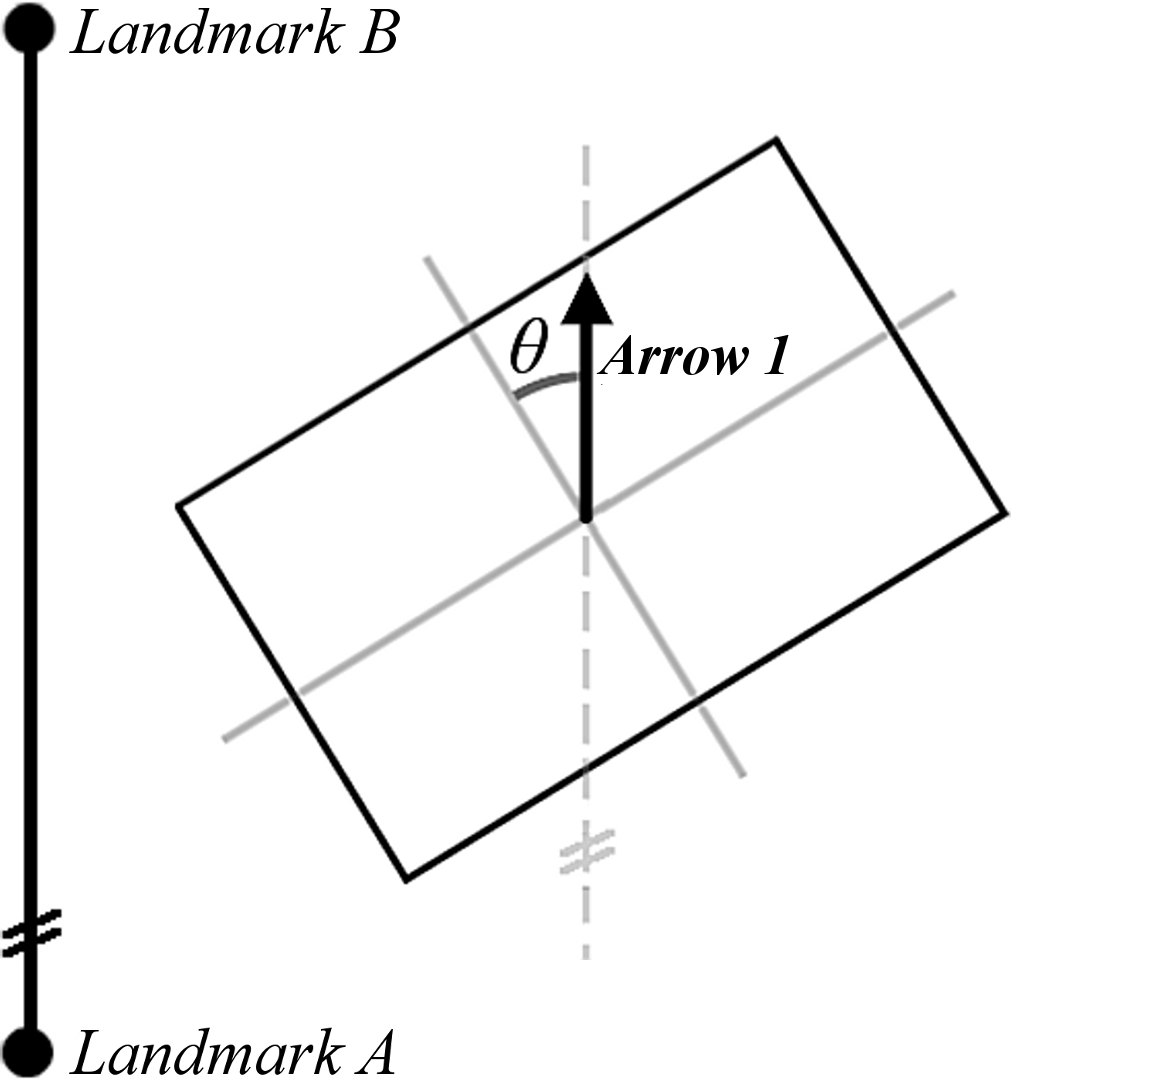
\includegraphics[width=0.4\textwidth]{figures/orientation_maths.png}
   \label{fig:orienTrig}
\end{figure}

The first of the three arrows used in the technique determines the orientation of the interface it is drawn on.
The user draws the arrow parallel to the imaginary line between the two landmarks.
The angle between this arrow and the local Y-axis of the interface, $\theta$ represents the orientation of the display as shown in Figure~\ref{fig:orienTrig}.
The user should draw this orientation arrow in the same direction on all the interfaces being located.
\textbf{$\theta$} can then be used to create a vector representing the real-world environment's Y-axis locally on the interface.
This can then be used in calculating the interface's physical position.

\begin{figure}[h]
   \centering
   \caption{Calculation of a interface's location.}
   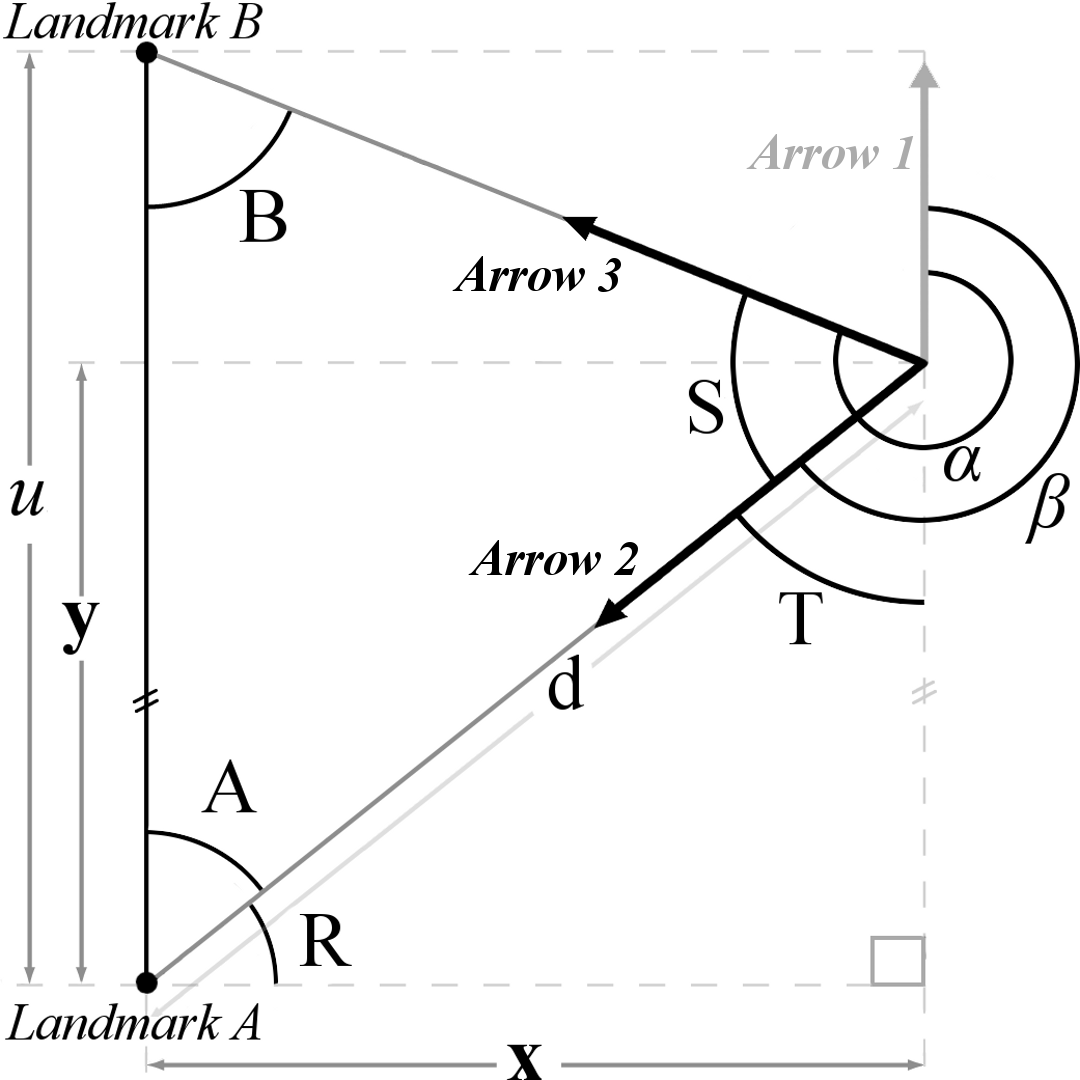
\includegraphics[width=0.475\textwidth]{figures/trig-illustration.png}
   \label{fig:trig}
\end{figure}

After drawing the orientation arrow the user is required to draw two further arrows which point directly to the landmarks (see Figure~\ref{fig:trig}).
Each of the arrows must point towards a separate landmark.
The angles of the user drawn arrows from the world's Y-axis, $\alpha$ and $\beta$, are used to determine the values used in calculating the location of the interface.
For each of these two arrows, the angle between the local y-axis of the interface and the arrow is summed with $\theta$ to derive $\alpha$ and $\beta$.

\begin{algorithm}[h]
\caption{Calculating the location of an interface.}
\label{algo:location}
\begin{algorithmic}
\STATE \textbf{getLocation}(${\alpha}, {\beta}$)
\INDSTATE[2] S = $\alpha - \beta$
\INDSTATE[2] T = $\beta$ - 180\degree
\INDSTATE[2] R = 90\degree - T
\INDSTATE[2] A = 90\degree - R
\INDSTATE[2] B = 180\degree - S - A
\INDSTATE[2] d = $\sin (B) * (u\ / \sin (S))$
\INDSTATE[2] x = $\sin (T) * (d\ / \sin (90\degree))$
\INDSTATE[2] y = $\sin (R) * (d\ / \sin (90\degree))$
\STATE {\emph{return}}\ x, y
\end{algorithmic}
\end{algorithm}

The angle between the two arrows, {\emph{S}}, is used in conjunction with the angle between one of the arrows and the local representation of the real world environment's Y-axis, {\emph{T}}, to determine the location of the interface.
Algorithm~\ref{algo:location} outlines the calculations involved in determining the \textbf{x} and \textbf{y} values of the interface's centre point in the physical environment.
The resulting values are relative to Landmark A's position as shown in Figure~\ref{fig:trig}.

This technique has a number of benefits over the alternatives of sensing technologies and direct measurements.
The technique only needs one known value before use; this is the distance between the landmarks.
Since it is a requirement of the technique that these landmarks are not moved, this value will not need to be re-measured.
Therefore, the technique can be performed relatively quickly once this measurement is obtained in comparison to measuring the locations of the interfaces directly.
This ability to be performed quickly without the need for repeated, time consuming measurements makes the technique suitable for any scenarios where the interfaces may be moved regularly.
Because of this the technique can be deemed {\emph{quick}}.

Because the technique does not rely on any additional technologies there is no additional cost for its implementation into a system.
This independence from additional hardware ensures that the technique is {\emph{inexpensive}} and {\emph{not encumbering}}.
Also, due to the technique's dependence on user inputs, rather than technologies, it is made suitable for use in environments where there may be many obstructions, such as the users themselves, around the interfaces.
If any immovable obstructions are present in the physical space between the interface and the reference points, a user can utilise their knowledge of the environment to make an informed placement of an arrow.
Therefore, the technique can be deemed {\emph{obstruction tolerant}}.

The technique's design does allow for its use on interfaces which do not utilise direct-touch inputs.
However, the ability to directly manipulate the arrows may be advantageous when trying to achieve an alignment between an on-screen arrow and a physical landmark. 
The act of aiming towards reference points allows for a form of direct feedback where the user can adjust the arrow until they believe they have the correct alignment.  
An indirect input device may draw a user's attention away from the interface, interrupting their concentration when aligning the arrows with landmarks.
The technique's suitability for direct-touch interfaces is enhanced by the fact that text entry, which would be required with other user input based techniques, through touch interfaces can be problematic due to their lack of tactile feedback~\cite{Weiss2009}.

This technique has been presented as an obstruction tolerant, quick, inexpensive and not encumbering solution.
However, its dependence on the accuracy of a user's judgement of direction has the implication that the positional information it produces may not be {\emph{accurate}}.
The inaccuracies in a user's input into the technique will result in the calculated position of the interface deviating from the interface's actual location.
This deviation between the calculated and actual interfaces locations could make this technique too inaccurate for use in some scenarios.
Therefore, it is important to discover how a user's inaccuracies when performing the technique affect the resulting value.

\section*{Study}\label{sec:study}

\begin{figure}[ht]
  \centering
   \caption{The positions and orientations of the markers and interfaces used in the user study.}
  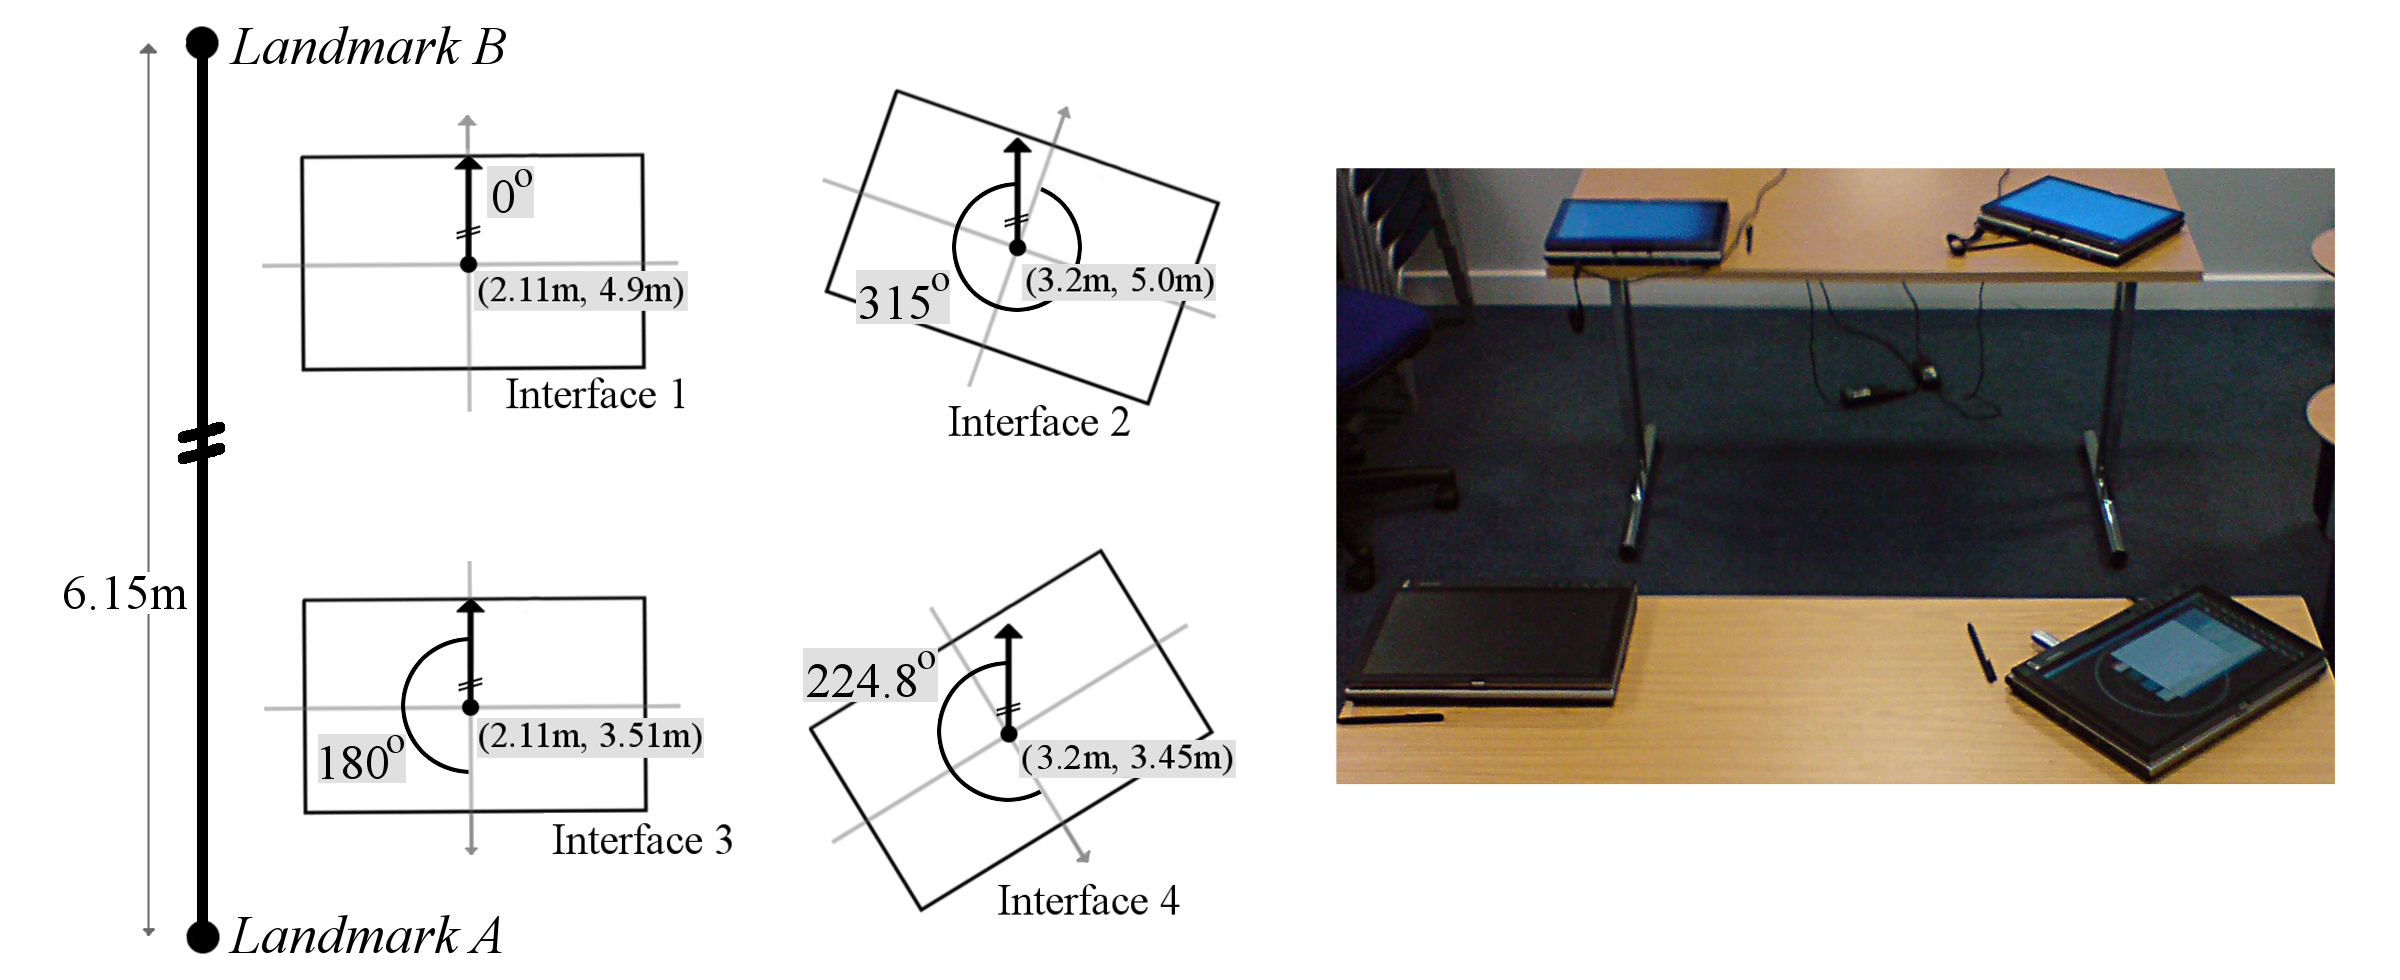
\includegraphics[width=0.9\textwidth]{figures/studyLayout.png}
   \label{fig:room}
\end{figure}

A study was conducted to determine how a user's accuracy affected the error of the presented technique's calculated interface positions.
The study focused on discovering whether the results given by the technique could be accurate enough for use in a specific scenario.
The technique was implemented into a software framework and deployed on four touch-screen tablet interfaces.

\subsection*{Implementation of the Technique}\label{sec:implementation}

Software for the study was constructed using the {\emph{SynergyNet}} multi-touch software framework~\cite{AlAgha2010}.
The framework utilises a number of third party libraries to support a wide range of functions such as networking, touch gesture recognition and multimedia support.
The technique was implemented as part of an application within the {\emph{SynergyNet}} framework which allowed for it to utilise a touch based input.

The arrows used in the implemented technique were designed to always originate from the centre of the interface.
The tail of an arrow remained in the centre of the interface while the participant could drag the arrowhead to any location on display.
The arrow being manipulated would therefore point from the centre of the interface towards the location of a participant's last relevant touch (relevant being defined as a touch within a certain distance of the arrowhead).
This allowed participants to determine the direction and length of the arrow.
The participant could reposition an arrowhead as much as they wanted.
Once a participant was finished establishing an arrow's direction they would then be expected to press a button on the interface to confirm their arrangement.

The technique first asked participants to draw a single arrow.
This arrow corresponds to arrow 1 in Figure~\ref{fig:orienTrig} which is used to establish the interface's orientation.
Once the participant confirmed their arrangement of this arrow they would then be asked to position two arrows together.
These are arrows 2 and 3 shown in figure~\ref{fig:trig}.
While each of the arrows for this stage of the technique is intended to point towards a landmark, the target for each arrow is not made explicit to the participant.
As long as each of the two arrows points at a different landmark it does not matter which landmark they point to.
The assumption is made in this implementation that all the interfaces are positioned in the space to the right of the line heading from landmark A to B.
Therefore, the arrow with the smallest clockwise angle from the environment's y-axis is arrow 2.
With this known, arrow 3 is known through the process of elimination.
When a participant was satisfied with the positioning of both these arrows they could then confirm their placement to complete the technique.

\subsection*{Study Design}\label{sec:design}

The tablet interfaces used in the study were positioned in the configuration shown in Figure~\ref{fig:room}.
This configuration was chosen to maximise the use of the four available interface devices in a non-symmetrical layout.
The orientations were chosen to include 
\begin{inparaenum}[(i)] 
\item orientations in line with the room's coordinate system (interfaces 1 and 3), 
\item reflection (between interfaces 1 and 3) and 
\item orientations not parallel to the room's coordinate system (interfaces 2 and 4).
\end{inparaenum}

Video recordings of the participants using the technique were made so that information regarding the timings and possible mistakes could be observed.
The application which the technique was implemented into was designed to record the local angle of any of the arrows drawn by a participant.
Any of the values used by the technique to calculate an interface's location were also recorded along with the resulting positional information.

Before the study took place direct measurements of the table's positions and orientations were made by the study organisers.
Using these values and the technique's calculations the angle of the arrows which would produce perfectly accurate positional information could be derived.
Comparing these optimal angles with the angles of user drawn arrows allowed for a participant's inaccuracy to be quantified.

The four tablet interface used in the study were identical.
Each tablet interface had a resolution of 1024 by 768 displayed on a 247mm by 185mm screen.

Two hypotheses were proposed prior to the study:

\begin{itemize}
\item[\textbf{Hypothesis 1}] {\emph{The error of the technique's result is proportional to the error user drawn arrows.}}

To support or disprove this hypothesis, the optimal angles of an interface were compared with the $\alpha$, $\beta$ and $\theta$ angles of the arrows drawn by the participants for each execution of the technique.
The deviation of a participant's arrows from their optimal angles could then be compared to the difference between the corresponding interface's calculated and actual location information (i.e. position and orientation).

\item[\textbf{Hypothesis 2}] {\emph{As participant's gain experience with the technique, their accuracy improves.}}

This hypothesis was derived from the observation that as users gain experience with an interaction technique their performance improves~\cite{Constantine1999}.
If user accuracy is found to influence the technique's result it is important to understand changes on it caused by practice.
The order of the tables on which the technique was performed was changed between participants.
This allowed any influences regarding the positioning of the interfaces to be distinguished from any learning effect the technique may have.
\end{itemize}


\section*{Results}\label{sec:results}  

13 participants took part in the study.
Each participant performed the technique 4 times, once on each interface resulting in 52 instances of the technique being executed.
All the participants were right-handed males who used computers daily and had at least some prior experience using the stylus interaction employed by the tablet interfaces.

\begin{figure}[h]
   \centering
   \caption{A scatter graph showing the correlation between the average inaccuracy of a participant's input into the technique and the error of the corresponding result.}
   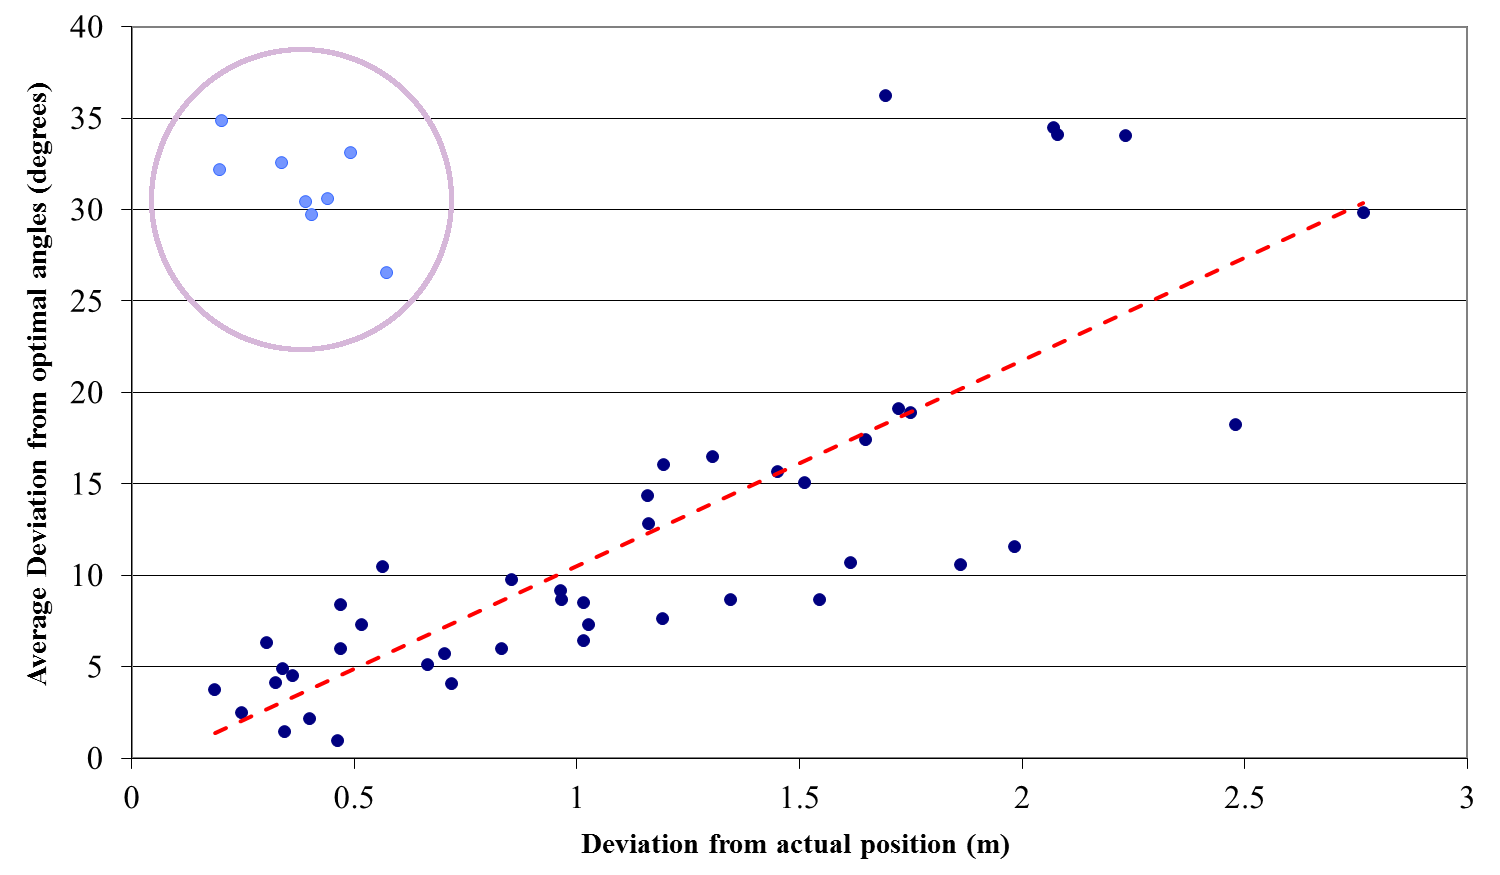
\includegraphics[width=0.6\textwidth]{figures/angle_deviation_scatter.png}
   \label{fig:scatter}
\end{figure}

Figure~\ref{fig:scatter} shows the average deviation of each participant's arrows from their optimal equivalents against the resulting positional information's average deviation from the actual location and orientation.
The graph in the figure indicates a general trend that as the average deviation from the optimum increases, the difference between an interface's actual and calculated positions increases.
This supports hypothesis 1 as a proportional relationship between the participant's inaccuracy and the error of the technique's result is demonstrated by the graph.
As noted on the graph there is a set of outlying data which does not conform to this trend, this is discussed in the \nameref{sec:discussion} section.

\begin{figure}[h]
   \centering
   \caption{A box plot graph showing the inaccuracy of participants against the number of times they have performed the technique.}
   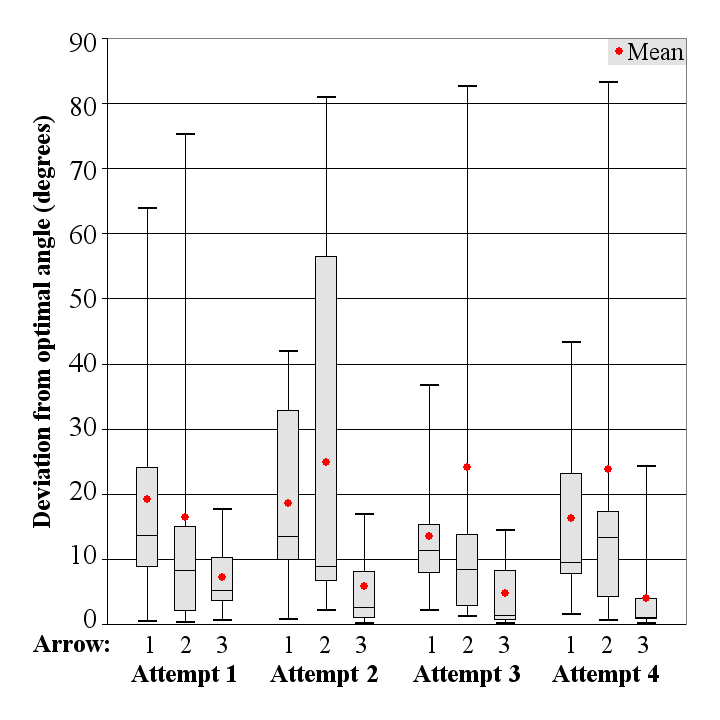
\includegraphics[width=0.6\textwidth]{figures/angle_deviation_boxplots.png}
   \label{fig:boxPlot}
\end{figure}

Figure~\ref{fig:boxPlot} shows the average deviation of participant drawn arrows from their equivalent optimal angles over the number of times a participant has performed the technique.
If hypothesis 2 was correct, the mean of participants' inaccuracies should decrease as the participants' experience with the technique increases.
However,  the graph shows there is no discernible improvement for any of the participant drawn arrows over the number of attempts made.
This indicates that there was no learning effect and that experience with the technique does not improve a participant's accuracy.
The evidence indicates that hypothesis 2 is incorrect.


\section*{Discussion}\label{sec:discussion}

\begin{figure}[bp]
   \centering
   \caption{A bar chart showing the relation between the magnitude of participant inaccuracies and the error of the technique's result.}
   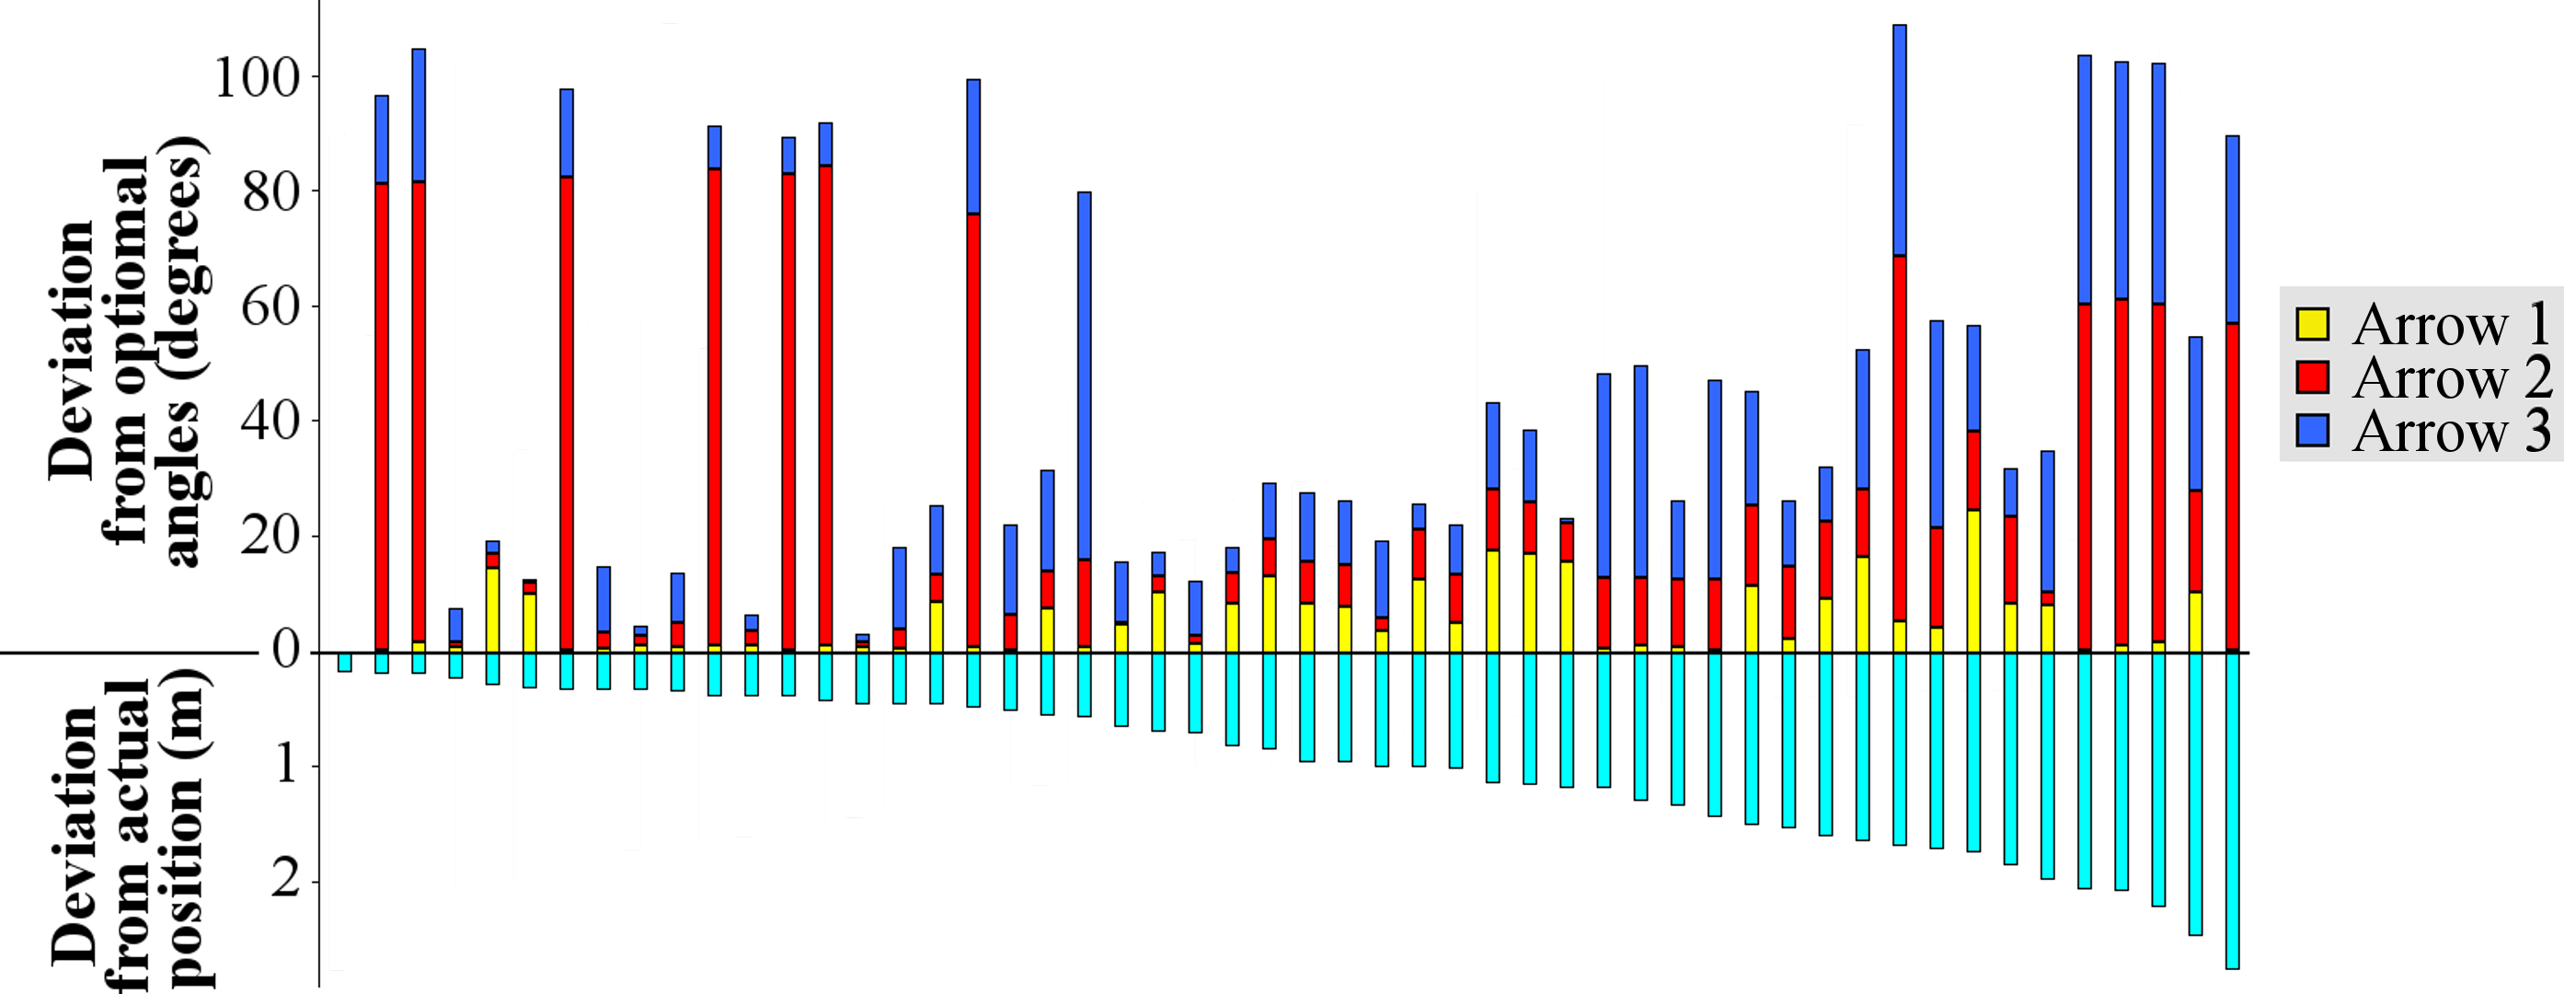
\includegraphics[width=0.9\textwidth]{figures/total_deviation_vs_angle_deviations.png}
   \label{fig:barReflect}
\end{figure}

As noted in the \nameref{sec:results} section, there is a subset of results which do not conform to the general trend of the data.
This subset consists of 8 results.
These outlying results are circled in Figure~\ref{fig:scatter} outside the grouping of the majority of data.
The data outside this subset of results implies that there is a proportional relationship between a user's accuracy and the error of the result.
However, these outlying results represent instances where a participant has been relatively inaccurate in comparison to other executions of the technique but a position with little deviation from the interface's actual position has been calculated.
This implies that the relationship between a user's inaccuracies and the error of the technique's result is more complex than hypothesis 1 states.

It is possible that one of the arrows used by the technique as an input has a greater influence over the result than the others.
The bars above the x-axis of the graph shown in Figure~\ref{fig:barReflect} represent deviation of participant drawn arrows from their corresponding optimums for all 52 instances of the technique being performed.
Under each of these bars, beneath the x-axis, is another bar which represents the error of the corresponding instance of the technique's result.
The graph highlights the general trend of participant's total inaccuracy increasing with the error of the result.
If any particular arrow input into the technique has a greater influence than the others then a relationship between the inaccuracies of the arrow and the result would be apparent.
For example, if arrow 1 had a significantly greater influence than arrows 2 and 3 then a correlation between the size of the participant inaccuracies when drawing this arrow and the magnitude of the error in the technique's result would be apparent.
However, no relation between the inaccuracy for a single arrow and the error of the technique's result is apparent in these results.

It is possible that a specific combination of arrows may have the greatest influence on the result, rather than a single arrow.
If this were true it would mean that one of the arrows would have comparatively little influence on the technique's result.
In circumstances where the participant inaccuracy for this inconsequential arrow is large, but is small for the other two arrows, the total deviation from the arrow optimums would not be proportional to the result's error.
This would account for the outlying data.
However, the data from the study does not support this as no relationship between the inaccuracy of two arrows and the error of the technique's result is apparent.

There is a further possibility that different individual arrows, or combination of arrows may have the greater influence in specific regions of the environment.
This could be due to the interface's proximity to the landmarks.
If an interface inhabits a region of the display where one of the landmarks used by the technique is significantly closer than the other, it is possible that the arrow pointing towards this landmark may hold a greater or lesser influence than in other regions of the environment.
Further study is required to discover if this theory is correct.
If true, knowledge of which arrow or combinations of arrows are the most influential in specific areas of an environment could be used to allow the system to reduce the impact of user inaccuracy.

Because users do not appear to become more accurate with experience, alternative methods of improving the accuracy of the technique will need to be employed.
Confidence ratings could be used to reduce the potential error of the technique's results.
Factors which influence a user's accuracy could be used to determine the initial confidence rating for an interface.
These ratings could then be used to assess whether a result is potentially accurate enough for use.
If not, the user could be asked to repeat the technique at this interface.
An average of the results from multiple executions of the technique on a specific interface could be used as the calculated position for further use by a system.
The deviation between the results could also be used to influence the confidence rating.
Since hypothesis 1 holds true, there is a proportional relationship between user accuracy and the size of the result's error.
A small deviation in the multiple results from a single interface would indicate that the user is being more accurate than a user producing a large deviation in their results.

As a user repeats the technique on an interface the confidence rating increases.
A greater confidence rating implies a higher probability of a more accurate calculated position.
However, one of the main strengths of this technique is the short amount of time it requires in comparison to the alternative of measuring the position of an interface directly.
Users were noted to take an average of 26.9 seconds per each performance of the technique in the study.
Repeating the technique increases the amount of time required to calculate the position on an interface.
It is important to consider the trade-off between the accuracy gained from repeats of the technique and the additional time required from users.
Using knowledge of where in an environment users may be less accurate, the number of times the technique is repeated could be kept to a minimum allowing for the best trade-off between time taken and accuracy.


\section*{Conclusions}\label{sec:conclusion}

Produced in this work is a technique that can employ a user's sense of direction to determine the location of an interface to a reasonable accuracy.
The technique offers a method of informing a system of the location and orientation of its affiliated interfaces without the need for additional technologies or time consuming measurements. 
This technique is obstruction tolerant, quick, inexpensive and not encumbering.
However, the accuracy of the technique is dependant on the accuracy of users.

The technique may be required to be made more accurate for use in some systems.
The accuracy of participants in the study was determined not to improve with practice.
Therefore attempts to improve the accuracy of users, and as a result reduce the error of the technique's result, cannot rely on users gaining experience with the technique.
Future work involving this technique will require discovering what influences a user's accuracy.
One such influence, discussed in the \nameref{sec:discussion} section, is the region of the environment relative to the landmarks which the display inhabits.
Other potential influences could include the distance between the interface and the landmarks, the number of landmarks used and the size of the interface.
The findings of any future studies concerning the technique could allow for improvements to its accuracy.
Knowledge of how accurate an execution of the technique is likely to be allows a confidence rating to be employed.
This confidence rating could be used to judge whether the result is usable for a specific scenario.
Through this confidence rating the best trade off could be discovered between the time the technique requires to be performed and the accuracy of the resulting calculated position.


%%%%%%%%%%%%%%%%%%%%%%%%%%%%%%%%%%%%%%%%%%%%%%
%%                                          %%
%% Backmatter begins here                   %%
%%                                          %%
%%%%%%%%%%%%%%%%%%%%%%%%%%%%%%%%%%%%%%%%%%%%%%

\begin{backmatter}

\section*{Competing interests}
  The authors declare that they have no competing interests.

\section*{Author's contributions}
    Text for this section \ldots

\section*{Acknowledgements}

This work was partially funded under the UK's EPSRC/ERSC Teaching and Learning Research Programme (TLRP) {\emph{SynergyNet}} project (RES-139-25-0400).

%%%%%%%%%%%%%%%%%%%%%%%%%%%%%%%%%%%%%%%%%%%%%%%%%%%%%%%%%%%%%
%%                  The Bibliography                       %%
%%                                                         %%
%%  Bmc_mathpys.bst  will be used to                       %%
%%  create a .BBL file for submission.                     %%
%%  After submission of the .TEX file,                     %%
%%  you will be prompted to submit your .BBL file.         %%
%%                                                         %%
%%                                                         %%
%%  Note that the displayed Bibliography will not          %%
%%  necessarily be rendered by Latex exactly as specified  %%
%%  in the online Instructions for Authors.                %%
%%                                                         %%
%%%%%%%%%%%%%%%%%%%%%%%%%%%%%%%%%%%%%%%%%%%%%%%%%%%%%%%%%%%%%

% if your bibliography is in bibtex format, use those commands:
\bibliographystyle{vancouver} % Style BST file (bmc-mathphys, vancouver, spbasic).
\bibliography{hccis2017}      % Bibliography file (usually '*.bib' )
% for author-year bibliography (bmc-mathphys or spbasic)
% a) write to bib file (bmc-mathphys only)
% @settings{label, options="nameyear"}
% b) uncomment next line
%\nocite{label}

% or include bibliography directly:
% \begin{thebibliography}
% \bibitem{b1}
% \end{thebibliography}

%%%%%%%%%%%%%%%%%%%%%%%%%%%%%%%%%%%
%%                               %%
%% Figures                       %%
%%                               %%
%% NB: this is for captions and  %%
%% Titles. All graphics must be  %%
%% submitted separately and NOT  %%
%% included in the Tex document  %%
%%                               %%
%%%%%%%%%%%%%%%%%%%%%%%%%%%%%%%%%%%

%%
%% Do not use \listoffigures as most will included as separate files

% \section*{Figures}
%   \begin{figure}[h!]
%   \caption{\csentence{Sample figure title.}
%       A short description of the figure content
%       should go here.}
%       \end{figure}

% \begin{figure}[h!]
%   \caption{\csentence{Sample figure title.}
%       Figure legend text.}
%       \end{figure}

%%%%%%%%%%%%%%%%%%%%%%%%%%%%%%%%%%%
%%                               %%
%% Tables                        %%
%%                               %%
%%%%%%%%%%%%%%%%%%%%%%%%%%%%%%%%%%%

%% Use of \listoftables is discouraged.
%%
% \section*{Tables}
% \begin{table}[h!]
% \caption{Sample table title. This is where the description of the table should go.}
%       \begin{tabular}{cccc}
%         \hline
%            & B1  &B2   & B3\\ \hline
%         A1 & 0.1 & 0.2 & 0.3\\
%         A2 & ... & ..  & .\\
%         A3 & ..  & .   & .\\ \hline
%       \end{tabular}
% \end{table}

%%%%%%%%%%%%%%%%%%%%%%%%%%%%%%%%%%%
%%                               %%
%% Additional Files              %%
%%                               %%
%%%%%%%%%%%%%%%%%%%%%%%%%%%%%%%%%%%

% \section*{Additional Files}
%   \subsection*{Additional file 1 --- Sample additional file title}
%     Additional file descriptions text (including details of how to
%     view the file, if it is in a non-standard format or the file extension).  This might
%     refer to a multi-page table or a figure.

%   \subsection*{Additional file 2 --- Sample additional file title}
%     Additional file descriptions text.


\end{backmatter}
\end{document}
